\begin{tikzpicture}[baseline=(current axis.center), scale=0.9]
\begin{axis}[
	y=1cm,
	ytick={1,2},
	yticklabels={Q1,Q3},
	xtick={1,2,3,4,5},
	xmax=5,
]
	\addplot+[boxplot] table [row sep=\\,y index=0] {
		Q1 \\ 4 \\ 4 \\ 3 \\ 3 \\ 4 \\ 4 \\ 4 \\ 4 \\ 3 \\
	};
	\addplot+[boxplot] table [row sep=\\,y index=0] {
		Q3 \\ 4 \\ 3 \\ 2 \\ 1 \\ 2 \\ 3 \\ 2 \\ 3 \\ 2 \\
	};
\end{axis}
\end{tikzpicture}
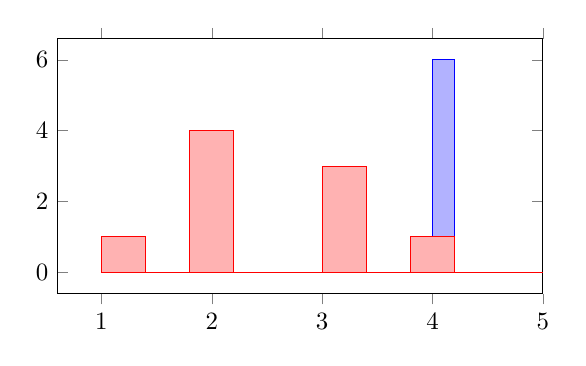
\begin{tikzpicture}[baseline=(current axis.center), scale=0.9]
\begin{axis}[
	ybar,
	y=0.5cm,
	xmax=5,
]
	\addplot+[hist] table [row sep=\\,y index=0] {
		Q1 \\ 4 \\ 4 \\ 3 \\ 3 \\ 4 \\ 4 \\ 4 \\ 4 \\ 3 \\
	};
	\addplot+[hist] table [row sep=\\,y index=0] {
		Q3 \\ 4 \\ 3 \\ 2 \\ 1 \\ 2 \\ 3 \\ 2 \\ 3 \\ 2 \\
	};
\end{axis}
\end{tikzpicture}
